
\chapter{Billeder}

At indsætte billeder i LaTeX er rimelig simpelt. Jeg vil her skrive den mest enkle måde, og derefter give et par muligheder for ændringer:\\

\indent \bs begin\{figure\}\\
\indent \bs includegraphics[width=1\bs linewidth]\{sti til billedet\}\\
\indent \bs end\{figure\}\\

\noindent
\bs begin og \bs end fortæller LaTeX at her skal vises en figur. Det er altid en god ide at have dem med, fordi billedet så bliver behandlet som en figur. \bs includegraphics er den kommando som faktisk henter billedet.\footnote{\bs includegraphics kommer fra pakken \emph{graphicx}.} [width=1\bs linewidth] fortæller LaTeX hvor bredt billedet må være (det betyder "1 * linjebredden"), her kan du selv eksperimentere med hvad der ser godt ud. \bs linewidth er hvor bred teksten er i dit dokument.\\
\noindent Her får du et eksempel:\\

\indent \bs begin\{figure\}\\
\indent \bs includegraphics[width=1\bs linewidth]\{billeder/madonna.jpeg\}\\
\indent \bs end\{figure\}\\

\begin{figure}[H]
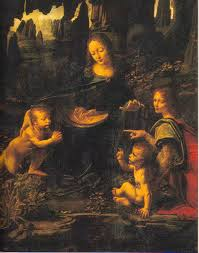
\includegraphics[width=1\linewidth]{billeder/madonna.jpeg}
\end{figure}

\section{Standard stuff}

Når jeg indsætter billeder, gør jeg som standard således:\\

\indent \bs begin\{figure\}[H]\\
\indent \bs centering\\
\indent \bs includegraphics[width=1\bs linewidth]\{sti\}\\
\indent \bs caption\{billedtekst\}\\
\indent \bs label\{fig:billedlabel\}\\
\indent \bs end\{figure\}\\

\noindent
[H] siger til LaTeX at billedet skal være der hvor jeg skriver det, og ikke må rykkes rundt.\footnote{[H] kommer fra pakken \emph{float}.} Normalt sætter LaTeX billeder således at siderne kan fyldes helt ud med tekst.

\noindent
\bs centering gør at LaTeX sætter billedet på midten af siden - du kan ikke se det i disse eksempler, men hvis billedet havde været mindre havde det gjort en forskel.

\noindent
\bs caption\{billedtekst\} sætter en tekst under billedet. Den gør også at billedet får vist sit tal.

\noindent
\bs label\{fig:billedlabel\} gør det nemmere at referere til billedet - se sektion  \ref{selvreferencer}. Når man giver figurer referencer, er det en god ide at skrive fig: foran - så er det nemmere at se hvad det er man refererer.\\

\noindent
Alt i alt ser det således ud:

\begin{figure}[H]
\centering
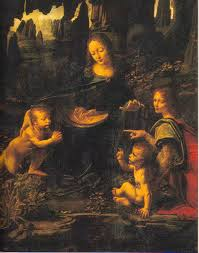
\includegraphics[width=1\linewidth]{billeder/madonna.jpeg}
\caption{"Madonna of the Rocks" af Leonardo da Vinci}
\label{fig:madonna_standard}
\end{figure}

\noindent
Den eneste forskel du kan se er altså figurteksten nedenunder :)

\section{Andet billedlayout}
\subsubsection{Rammer}
Hvis du gerne vil have en ramme rundt om et billede, kan du skrive \bs includegraphics ind i en \bs fbox:\\

\indent \bs begin\{figure\}\\
\indent ... \\
\indent \bs fbox\{\bs includegraphics[width=.8\bs linewidth]\{sti til billede\}\}\\
\indent ... \\
\indent \bs end\{figure\}\\

\begin{figure}[H]
\centering
\fbox{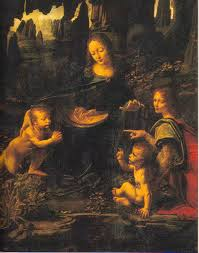
\includegraphics[width=.8\linewidth]{billeder/madonna.jpeg}}
\caption{Madonna med ramme}
\label{fig:madonna_ramme}
\end{figure}

\noindent
Hvis du vil have mere avancerede rammer, vil jeg foreslå at du søger på nettet. Der findes en pakke som hedder \emph{mdframed} som er sej, men det er for meget at skrive om her.

\subsubsection{Text-wrap}
At få teksten til at kunne stå rundt om billedet er en lidt større operation, og sjældent nødvendig i akademiske tekster. Se dette link for en beskrivelse af hvordan man kan gøre: \url{http://en.wikibooks.org/wiki/LaTeX/Floats,_Figures_and_Captions}.

\section{PDF'er}
Hvis man gerne vil inkludere en pdf fil eller et par sider fra den, skal man bruge følgende kommando:\\

\indent \bs includepdf[pages=\{sidetal\}]\{sti til pdf'en\}\\

\noindent
I "sidetal" feltet kan du skrive, for eksempel \{1, 3, 5-9\}, og du vil i så fald få side 1, 3 og 5 til 9 med. Hvis du vil have alle siderne med, skriver du \{-\}. Pdf sider vil altid stå på en side for sig.\footnote{\bs includepdf kommandoen kommer fra pakken \emph{pdfpages}.}
